%%%%%%%%%%%%%%%%%%%%%%%%%%%%%%%%%%%%%%%%%%%%%%%%%%%%%%%%%%%%%%%%%%%%%%%
% Thema: Poster SHOCK
% Autor: Manuel Gageik
%%%%%%%%%%%%%%%%%%%%%%%%%%%%%%%%%%%%%%%%%%%%%%%%%%%%%%%%%%%%%%%%%%%%%%%
%
\documentclass[a0,portrait]{a0poster}
%\documentclass[portrait,a0,posterdraft]{a0poster}
%
%%%%%%%%%%%%%%%%%%%%%%%%%%%%%%%%%%%%%%%%%%%%%%%%%%%%%%%%%%%%%%%%%%%%%%%
% Paket zum Erzeugen der Spalten
\usepackage{multicol}

%%%%%%%%%%%%%%%%%%%%%%%%%%%%%%%%%%%%%%%%%%%%%%%%%%%%%%%%%%%%%%%%%%%%%%%
% Eingabekodierung
\usepackage[ansinew]{inputenc}
\usepackage[T1]{fontenc}
\usepackage{ae} %wenn Ulaute nicht gehen

\usepackage[ngerman]{babel}
%\begin{übler Trick um die Orinalüberschrift zu unterdrücken}
\addto{\captionsngerman}{\renewcommand*{\refname}{}} %Literaturüberschfit unterdrücken
%\ende{übler Trick}

%%%%%%%%%%%%%%%%%%%%%%%%%%%%%%%%%%%%%%%%%%%%%%%%%%%%%%%%%%%%%%%%%%%%%%%
% für Farbe
\usepackage{color} 
\definecolor{darkgreen}{rgb}{0,0.5,0} 
\definecolor{darkblue}{rgb}{0,0,0.5}

%%%%%%%%%%%%%%%%%%%%%%%%%%%%%%%%%%%%%%%%%%%%%%%%%%%%%%%%%%%%%%%%%%%%%%%
% Mathepaket
\usepackage{amsmath} 

%%%%%%%%%%%%%%%%%%%%%%%%%%%%%%%%%%%%%%%%%%%%%%%%%%%%%%%%%%%%%%%%%%%%%%%
% Ist für Boxen (wie das hier benutzte Ovalbox) zuständig
\usepackage{fancybox}

%%%%%%%%%%%%%%%%%%%%%%%%%%%%%%%%%%%%%%%%%%%%%%%%%%%%%%%%%%%%%%%%%%%%%%%
% Graphikpaket, ermöglicht png, jpg und pdf bilder
\usepackage{graphicx}

%%%%%%%%%%%%%%%%%%%%%%%%%%%%%%%%%%%%%%%%%%%%%%%%%%%%%%%%%%%%%%%%%%%%%%%
% Seiteneinstellungen
\renewcommand\baselinestretch{1.35}
\parskip=0.5\baselineskip

\parindent0mm %Einrücktiefe der ersten Zeile eines Absatzes
\topmargin-28pt
\marginparwidth0mm

%Ränder rechts/links
\oddsidemargin-13pt
\evensidemargin-13pt
\textwidth785mm
%\textheight1140mm

%%%%%%%%%%%%%%%%%%%%%%%%%%%%%%%%%%%%%%%%%%%%%%%%%%%%%%%%%%%%%%%%%%%%%%%
% Eigene Definitionen zur Erleichterung des Satzes
\newcommand{\spaltenbreite}{25}   % Spaltenbreite für Bilder
\newcommand{\bildbreite}{25cm}    % Einheitliche Bildbreite

%%%%%%%%%%%%%%%%%%%%%%%%%%%%%%%%%%%%%%%%%%%%%%%%%%%%%%%%%%%%%%%%%%%%%%%
% Box- und Spalteneinstellungen
\setlength{\fboxrule}{3.25mm} %Definiert die Linienstärke für nachfolgende fbox- und framebox-Befehle
\setlength{\fboxsep}{5mm} %Abstand zwischen Rahmen und Text bei den /fbox und /framebox Befehlen.
\setlength{\columnsep}{15mm}     %Spaltenabstand
\setlength{\columnseprule}{1pt}  %Balken zwischen Spalten {0pt}->keine Balken

%%%%%%%%%%%%%%%%%%%%%%%%%%%%%%%%%%%%%%%%%%%%%%%%%%%%%%%%%%%%%%%%%%%%%%%
% Einheitslänge für picture-Umgebungen
%\setlength{\unitlength}{1.0cm}
\unitlength1cm

%%%%%%%%%%%%%%%%%%%%%%%%%%%%%%%%%%%%%%%%%%%%%%%%%%%%%%%%%%%%%%%%%%%%%%%
% Grafikpfad, hier liegen alle Bilder
%\graphicspath{{images/}}

%%%%%%%%%%%%%%%%%%%%%%%%%%%%%%%%%%%%%%%%%%%%%%%%%%%%%%%%%%%%%%%%%%%%%%%
% Zaehler fuer lineale. Sie werden gebraucht, wenn das Linealmacro
% included wird
\newcounter{skalax}
\newcounter{skalay}


\begin{document}

%%%%%%%%%%%%%%%%%%%%%%%%%%%%%%%%%%%%%%%%%%%%%%%%%%%%%%%%%%%%%%%%%%%%%%%
% Kopf, hier funktioniert alles mit 'put'
%%%%%%%%%%%%%%%%%%%%%%%%%%%%%%%%%%%%%%%%%%%%%%%%%%%%%%%%%%%%%%%%%%%%%%%
%\parbox{\textwidth}
%{
  \begin{center}
    \vspace*{0.006\textheight}
   % Titel und Autor
    {\Huge \textbf{SHOCK}\\}%[0.03\textheight]
    \vspace*{0.018\textheight}
    {\LARGE \textbf{\textbf{S}tructured \textbf{H}igh-\textbf{O}rder \textbf{C}omputational \textbf{K}ernel}\\}
    {\Large for Direct Numerical Simulation of compressible flows}
    %\vspace*{0.018\textheight}
    %{\Large \textbf{for Direct Numerical Simulation of compressible flow}}
  \end{center}
  % Logos einbinden (per Hand plazieren)
  \begin{picture}(0,0)
    \put(1.0 , 7.0){
\includegraphics[height=40mm]{SWL_Logo.JPG}}
    \put(2.4 , 6.0){\large \textbf{Prof. Dr.-Ing Herbert Olivier}}
    \put(62.0 , 10.0){\large \textbf{Section Numerical Simulation}}
    \put(62.0 , 8.5){\large Prof.Dr.habil.(RUS) I. Klioutchnikov}
    \put(62.0 , 7.0){\large Dipl.-Ing. M. Gageik}
    \end{picture}
%}

%%%%%%%%%%%%%%%%%%%%%%%%%%%%%%%%%%%%%%%%%%%%%%%%%%%%%%%%%%%%%%%%%%%%%%%
% Einstellung des Eckenradius' der ovalen Boxen (\Ovalbox)
\cornersize*{5mm}


\linethickness{0.1mm}
\setlength{\fboxrule}{2.25mm}

%%%%%%%%%%%%%%%%%%%%%%%%%%%%%%%%%%%%%%%%%%%%%%%%%%%%%%%%%%%%%%%%%%%%%%% 
% neuer Kasten
\Ovalbox
{
  \parbox{\textwidth}{
\includegraphics[width=0.98\textwidth]{SHOCK_3b.png}    
  }
}

%%%%%%%%%%%%%%%%%%%%%%%%%%%%%%%%%%%%%%%%%%%%%%%%%%%%%%%%%%%%%%%%%%%%%%% 
% neuer Kasten
\Ovalbox
{
  \parbox{\textwidth}{
\includegraphics[width=0.98\textwidth]{SHOCK_1b.png}    
  }
}

%%%%%%%%%%%%%%%%%%%%%%%%%%%%%%%%%%%%%%%%%%%%%%%%%%%%%%%%%%%%%%%%%%%%%%%
% neuer Kasten
\vspace*{0.002\textheight}
\Ovalbox
{
  \parbox{\textwidth}{
    \begin{multicols}{3}
    
\textbf{Direct Numerical Simulation}
\newline
\begin{itemize}
\item flow configurations:
\begin{itemize}
\item compressible, unsteady
\item viscous (Navier-Stokes) or inviscid (Euler)
\item three-dimensional, two-dimensional rotational symmentric or two-dimensional
\item curvilinear coordinates (including subzones with rotated coordinate systems)
\end{itemize}
\item high-order shock capturing schemes:
\begin{itemize}
\item $5^{th}$ and $9^{th}$ order WENO scheme (inviscid)
\item Lax-Friedrichs flux-vector splitting
\item $6^{th}$ and $10^{th}$ order central scheme (viscous)
\item $3^{rd}$ and $4^{th}$ order Runge-Kutta (time)
\newline
\newline
\end{itemize}
\end{itemize}      

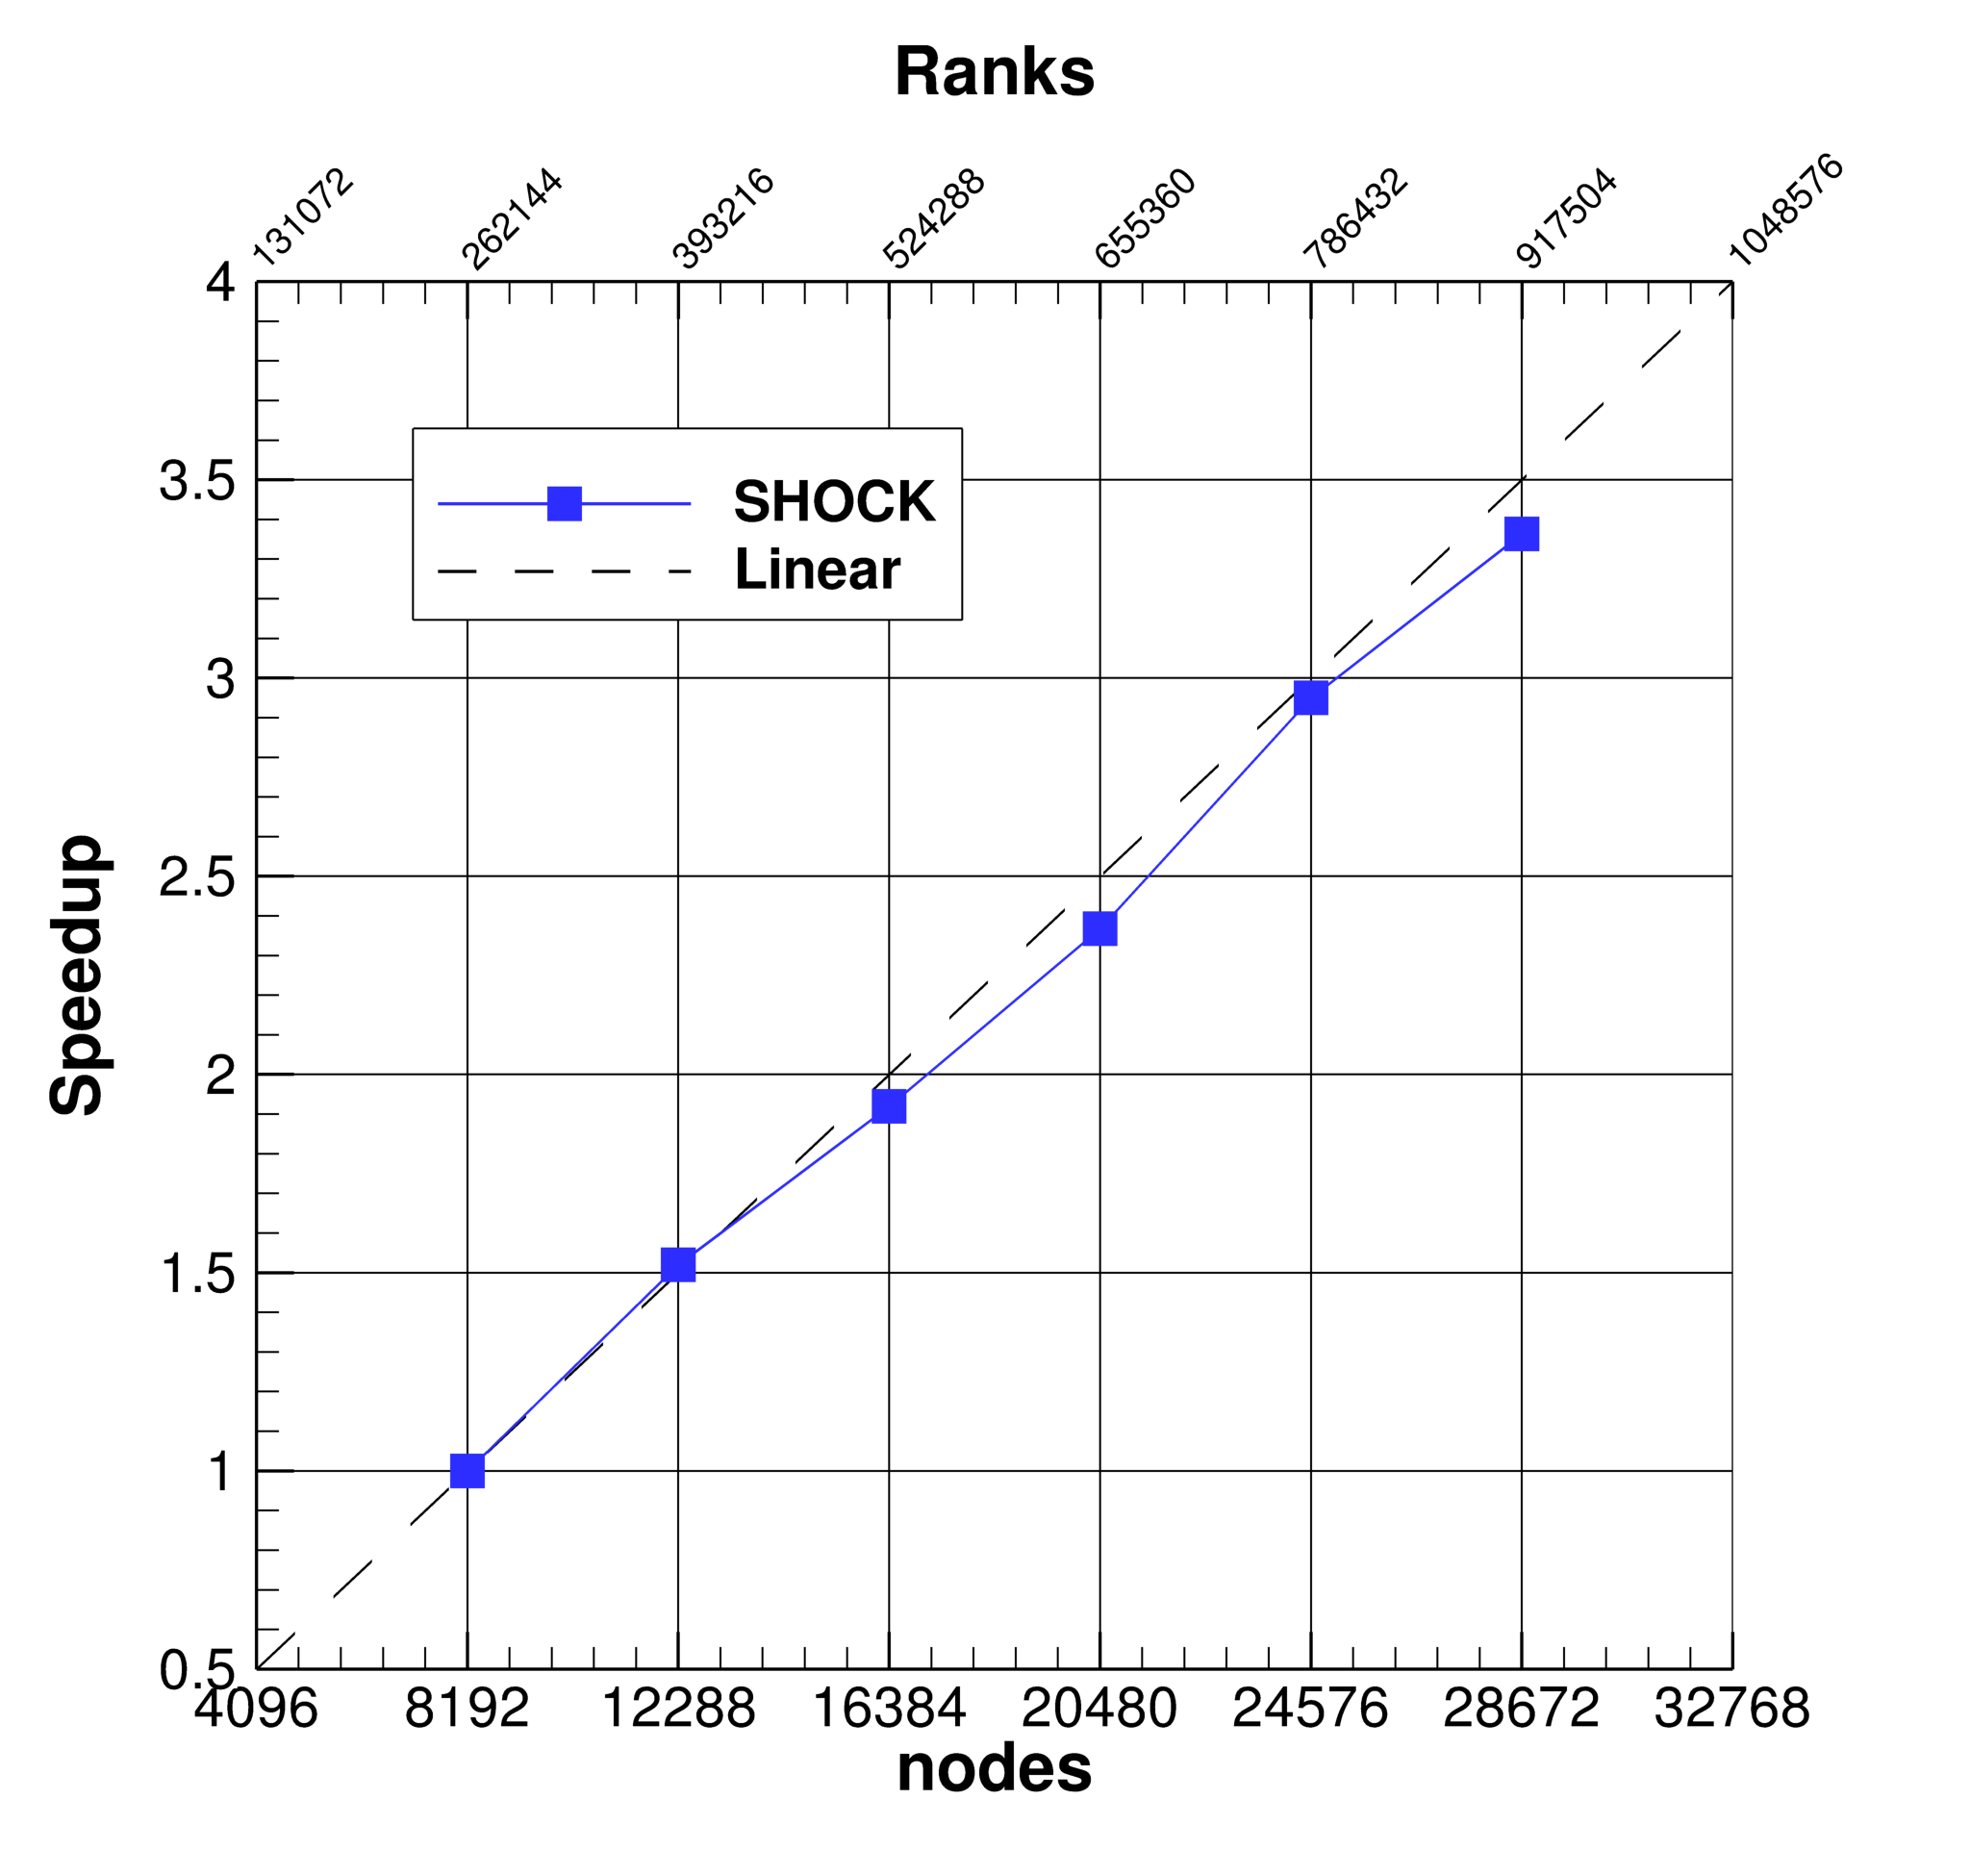
\includegraphics[height=260mm]{Scaling.png}

\textbf{Scalability}
\begin{itemize}
\item SHOCK is member of the \textbf{High-Q Club} \newline (Highest Scaling Codes on JUQUEEN [FZ J\"{u}lich])
\item 458,752 cores (1,835,008 compute threads) \newline on BlueGene/Q (JUQUEEN)
\end{itemize}

\textbf{Programming language}
\begin{itemize}
\item C
\item pure MPI (asynchronous)
\item I/O in parallel HDF5 (CGNS)
\end{itemize}

\textbf{Tested on platform}
\begin{itemize}
\item Bull-Cluster (RWTH Aachen)
\item BlueGene/Q (FZ J\"{u}lich)
\end{itemize}

\textbf{Application developers}
\begin{itemize}
\item Gageik, Manuel, Dipl.-Ing. \newline gageik@swl.rwth-aachen.de 
\item Klioutchnikov, Igor, Prof. Dr.rer.nat. habil. (RUS) \newline klioutchnikov@swl.rwth-aachen.de 
\end{itemize}
      
    \end{multicols}
  }
}


\end{document}